\part{Ejercicio 3}
\section{Enunciado}
Dado un arreglo de $n$ elementos en el que hay un elemento que aparece m'as de la mitad de las 
veces, encontrar la moda, es decir, el valor que aparece m'as veces.

\section{Desarrollo}
\paragraph{}
La primera idea para abordar este problema fue la de ordenar el arreglo y contar la cantidad 
de apariciones guardando el elemento con m'as apariciones. Esta primera idea no tuvo mucha 
aceptaci'on ya que se observ'o que el orden requerido para ordenar dicho arreglo era $O(n*log$ $n)$ 
y pensamos que deb'iamos buscar un orden mejor.
\paragraph{}
Una mejora a este procedimiento fue notar que la moda en un arreglo con las caracter'isticas
dadas por el problema coincide con el elemento $n/2$ del arreglo ordenado. Por lo tanto, 
si se ordena el arreglo, en vez de contar apariciones basta con tomar el elemento $n/2$ para 
obtener la moda. Sin embargo, esta mejora tambi'en requiere que el arreglo sea ordenado, y por
lo tanto, al igual que la idea anterior, qued'o descartado por tener un orden de complejidad
demasiado alto.
\paragraph{}
Investigando sobre el tema se encontr'o el algoritmo de Loyd-Pratt-Rivest-Tarjan, que permite 
encontrar la mediana (mediana en el sentido de elemento del medio, que si el arreglo tiene una 
cantidad impar de elementos coincide con la mediana estad'istica, si no, no es exactamente el 
mismo concepto; pero lo usamos para abreviar) de un arreglo en orden lineal sin necesidad de ordenarlo.
\paragraph{}
El algoritmo se basa en el uso de un pivote para partir el arreglo y quedarse solo con la parte donde se 
puede encontrar la mediana. Es necesario para tener orden lineal poder encontrar un buen pivote 
en un orden a lo sumo lineal. El algoritmo resuelve esto partiendo el arreglo principal en arreglos
de 5 elementos, tomando la mediana de 'estos y luego tomando una seudomediana a partir de dicha ``mediana''. 
Se puede demostrar que este procedimiento permite encontrar la mediana en un orden lineal. Esta 
soluci'on se descart'o ya que su implementaci'on era bastante complicada, y la demostraci'on del orden de complejidad tambi'en lo era.
\paragraph{}
Se busc'o entonces otra forma de  obtener un orden lineal aprovechando que la frecuencia de la moda 
era mayor a la mitad. La idea que tuvimos consiste b'asicamente en recorrer el arreglo sirvi'endose de 
dos 'indices. Si se encuentran dos elementos iguales, se incrementa uno de los 'indices (en adelante $j$) 
y se deja inm'ovil al otro (en adelante $i$) en la posici'on donde se encuentra. Si se encuentran dos 
elementos diferentes, estos son tachados (para esto se utiliza una marca sobre un arreglo de posiciones booleanas). 
\paragraph{}
Luego se avanza $i$ hasta que llegue a una posici'on sin tachar y se hace lo propio con $j$ hasta llegar 
a una posici'on sin tachar pero que tambi'en sea mayor que $i$. El ciclo termina cuando $j$ excede el l'imite 
del arreglo. Se devuelve entonces el valor donde qued'o parado el 'indice $i$. 
En cada paso el algoritmo ``tacha'' dos elementos que no son la moda, o uno que es la moda y otro que no. 
De esta forma solo terminan sobreviviendo algunos elementos de la moda. Al terminar el ciclo, los elementos
sin tachar desde $i$ hasta el final del arreglo son iguales. Entonces podr'ian o bien ser moda o ser elementos 
distintos a la moda. Sin embargo, esto 'ultimo no puede ocurrir ya que la frecuencia de la moda es como m'inimo 
$n/2+1$, entonces que eso ocurra implicar'ia que tach'e por lo menos $2*(n/2+1)$ elementos pero $2*(n/2+1) > n$.
\paragraph{}
El siguiente es un ejemplo de la aplicaci'on del algoritmo:\\
\begin{figure}[H]
\centering
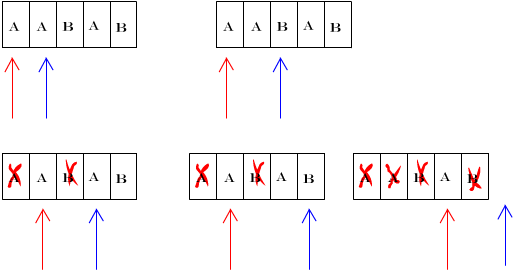
\includegraphics[scale=0.7]{./ejemplo.png}
\caption{Ejemplo de la aplicaci'on del algoritmo}
\end{figure}
\paragraph{}
En el ejemplo, al principio como estamos parados en dos elementos iguales, solo se avanza el 'indice de adelante. 
Como ahora son diferentes, se tachan y se avanzan los 'indices. Nuevamente son iguales por lo que s'olo 
se avanza el de adelante. Se tacha nuevamente un par de elementos, y al avanzar el 'indice de adelante se 
termina el arreglo. La moda es entonces el elemento donde est'a parado el 'indice de atr'as.
Este algoritmo fue finalmente el que se adopt'o como soluci'on ya que nos garantizaba el orden lineal 
buscado y su implementaci'on era simple.

\section{Pseudoc'odigo}
\begin{algorithm}
\caption{Halla la moda $moda$ del arreglo $a$}
\begin{algorithmic}[1]
\STATE indiceDeAtras $\textcolor{orange}{\leftarrow}$ 0
\STATE indiceDeAdelante $\textcolor{orange}{\leftarrow}$ 0
\STATE tachados: [bool] \COMMENT{los elementos de tachados inicializan en false}\\

\WHILE{indiceDeAdelante $\textcolor{orange}{<}$ tamanio\textcolor{magenta}{(}a\textcolor{magenta}{)}}
    \IF{$a_{indiceDeAtras}$ $\textcolor{orange}{\neq}$ $a_{indiceDeAdelante}$}
        \STATE tachados $\textcolor{orange}{\leftarrow}$ tachar ambos elementos //donde: tachar i es asignar con true en el elemento iesimo de tachados
        \WHILE{\textcolor{magenta}{(}indiceDeAtras $\textcolor{orange}{<}$ tamanio\textcolor{magenta}{(}a\textcolor{magenta}{)} \textcolor{orange}{\&} \textcolor{magenta}{(}indiceDeAtras no fue tachado\textcolor{magenta}{)}}
            \STATE indiceDeAtras $\textcolor{orange}{\leftarrow}$ indiceDeAtras \textcolor{orange}{+} 1
        \ENDWHILE
        \WHILE{indiceDeAdelante $\textcolor{orange}{<}$ tamanio\textcolor{magenta}{(}a\textcolor{magenta}{)} \textcolor{orange}{\&} \textcolor{magenta}{(}indiceDeAdelante no fue tachado $\textcolor{orange}{|}$ indiceDeAdelante $\leq$ indiceDeAtras\textcolor{magenta}{)}}
            \STATE indiceDeAdelante $\textcolor{orange}{\leftarrow}$ indiceDeAdelante \textcolor{orange}{+} 1
        \ENDWHILE
    \ELSE
        \STATE indiceDeAdelante $\textcolor{orange}{\leftarrow}$ indiceDeAdelante \textcolor{orange}{+} 1
    \ENDIF

\ENDWHILE
\STATE $moda \textcolor{orange}{\leftarrow}$ $a_{indiceDeAtras}$
\end{algorithmic}
\end{algorithm}


\newpage
\section{C'alculo de complejidad}
Para hacer el c'alculo de complejidad utilizamos el modelo uniforme pues consideramos, al igual que con 
el ejercicio anterior, que lo fundamental a la hora de estudiar el orden pasa por la cantidad de elementos 
a estudiar, y no por los valores de los mismos. Por ende es razonable asumir que el costo de operar
con los n'umeros propiamente dichos es constante.
\paragraph{}
Considerando esto, afirmamos que si el arreglo tiene $n$ elementos, el tama\~{n}o de la entrada es $n$.\\
Pensando en el comportamiento que tiene el algoritmo, vemos que siempre recorremos el arreglo hacia adelante 
y nunca volvemos hacia atr'as. Es por esta raz'on que si bien hay ciclos anidados (dentro del de la l'inea 
4 tenemos al de la l'inea 7 y el de la l'inea 10) el algoritmo es $O(n)$.
\paragraph{}
El ciclo de la l'inea 7 usa indiceDeAtras para recorrer el arreglo, ahora la guarda del ciclo es:\\

indiceDeAtras $<$ tamanio(a) $\&$ (indiceDeAtras no fue tachado)\

\paragraph{}
Entonces podemos ver que este ciclo, dado que $i$ no se reinicia, solo recorre el arreglo a lo sumo una 
vez en todos los ciclos del de la l'inea 4. Es decir, si el ciclo principal hace $k$ iteraciones y llamamos 
$iterAtras_t$ al numero de iteraciones del ciclo de la l'inea 7 en la iteraci'on t del ciclo principal, vale que:

$$\sum_{t=1}^{k}iterAtras_t \leq n$$

ya que en el momento en que $i$ se hace $n$ el ciclo interno no itera m'as.
\paragraph{}
La situaci'on del ciclo de la l'inea 10 es similar, en este caso la guarda es:\\

indiceDeAdelante $<$ tamanio(a) $\&$ (indiceDeAdelante no fue tachado $\|$ indiceDeAdelante $\leq$ indiceDeAtras)

\paragraph{}
Es decir que el n'umero de iteraciones est'a en principio acotado por $n$. Por otro lado la variable $indiceDeAdelante$, 
que no se reinicia, es la que establece la condici'on de salida del ciclo principal. Si, an'alogamente a como hicimos 
antes, el ciclo principal hace $k$ iteraciones y llamamos $iterAdel_t$ al n'umero de iteraciones del ciclo de 
la l'inea 10, se puede ver que:

$$\sum_{t=1}^{k}iterAdel_t \leq n$$

porque en el momento en que el 'indice de adelante llega a n, ninguno de los ciclos itera mas.

Y en particular si definimos:\\

$beta(b) =$ if b then 1 else 0 \\

Y definimos $indiceAtras_t$, $indiceAdelante_t$ a los valores de dichos 'indices en la iteraci'on t, tenemos que:

$$n=\sum_{t=0}^{k}beta(a[indiceDeAtras_t] == a[indiceDeAdelante_t])+ iterAdel_t$$

ya que o indiceDeAdelante se incrementa en una unidad porque los elementos eran iguales, o itera el ciclo interno.\\

\paragraph{}
Viendo esto es de notar que tanto indiceDeAtras como indiceDeAdelante solo recorren el arreglo una vez. 
\paragraph{}
Por lo tanto el algoritmo tiene un orden de complejidad lineal, es decir $O(n)$.
\paragraph{}
Observando el pseudoc'odigo, tambien notamos como en la medida que aumenta el n'umero de apariciones de la 
moda (y por lo tanto la guarda del $if$ de la l'inea 5 se haga falsa en m'as oportunidades) m'as r'apido 
deber'ia andar el algoritmo, ya que s'olo se incrementa $indiceDeAdelante$. En vista de 'esto, si los elementos 
del arreglo son todos iguales, el algoritmo hace solo una pasada, mientras que en el peor de los casos, 
hace dos pasadas completas.

\section{An'alisis Experimental}
\subsection{Experiencias realizadas}
\paragraph{}
Nuevamente para este algoritmo se decidi'o medir tanto la cantidad de operaciones como el tiempo en funci'on de la cantidad de 
elementos del arreglo, con la intenci'on de confirmar nuestro analisis te'orico. Para ello se generaron arreglos de largo creciente 
con elementos al azar (distribuci'on uniforme) respetando que la frecuencia de la moda sea de por lo menos $n/2+1$.
\paragraph{}
Por otro lado para observar la influencia de la frecuencia de la moda en el comportamiento del algoritmo se hicieron corridas de prueba
para un $n$ fijo aumentando la frecuencia y midiendo la cantidad de operaciones y el tiempo insumido.
\paragraph{}
Adem'as, en algunos casos fue posible utilizar la t'ecnica de cuadrados m'inimos para dar una funci'on 
que aproxime el comportamiento observado experimentalmente. En dichos casos, la ecuaci'on de $f(x)$ se encuentra en el gr'afico.

\subsection{Gr'aficos}

\begin{figure}[H]
\centering
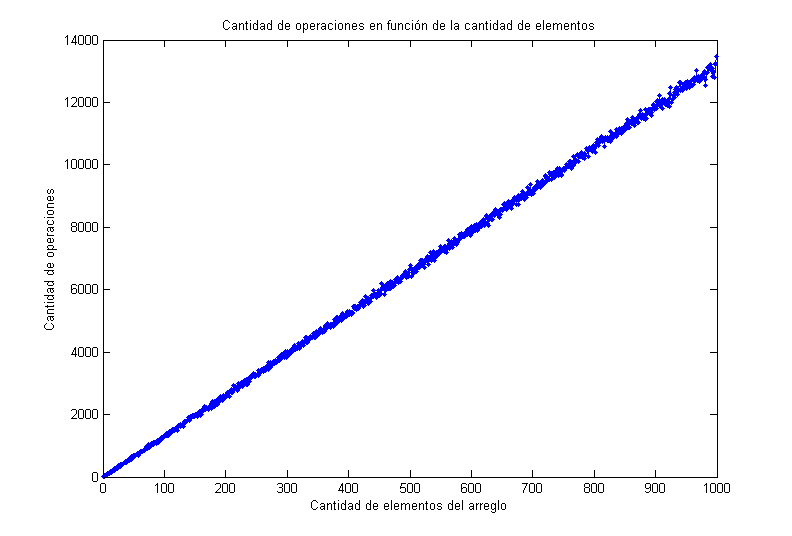
\includegraphics[scale=0.7]{../../codigo/ejercicio3/benchmark/graficos/corridas_aleatorias_n_creciente/grafico.png}
\caption{Cantidad de operaciones en funci'on del tama\~{n}o del arreglo}
\label{Ej3fig1}
\end{figure}

\begin{figure}[H]
\centering
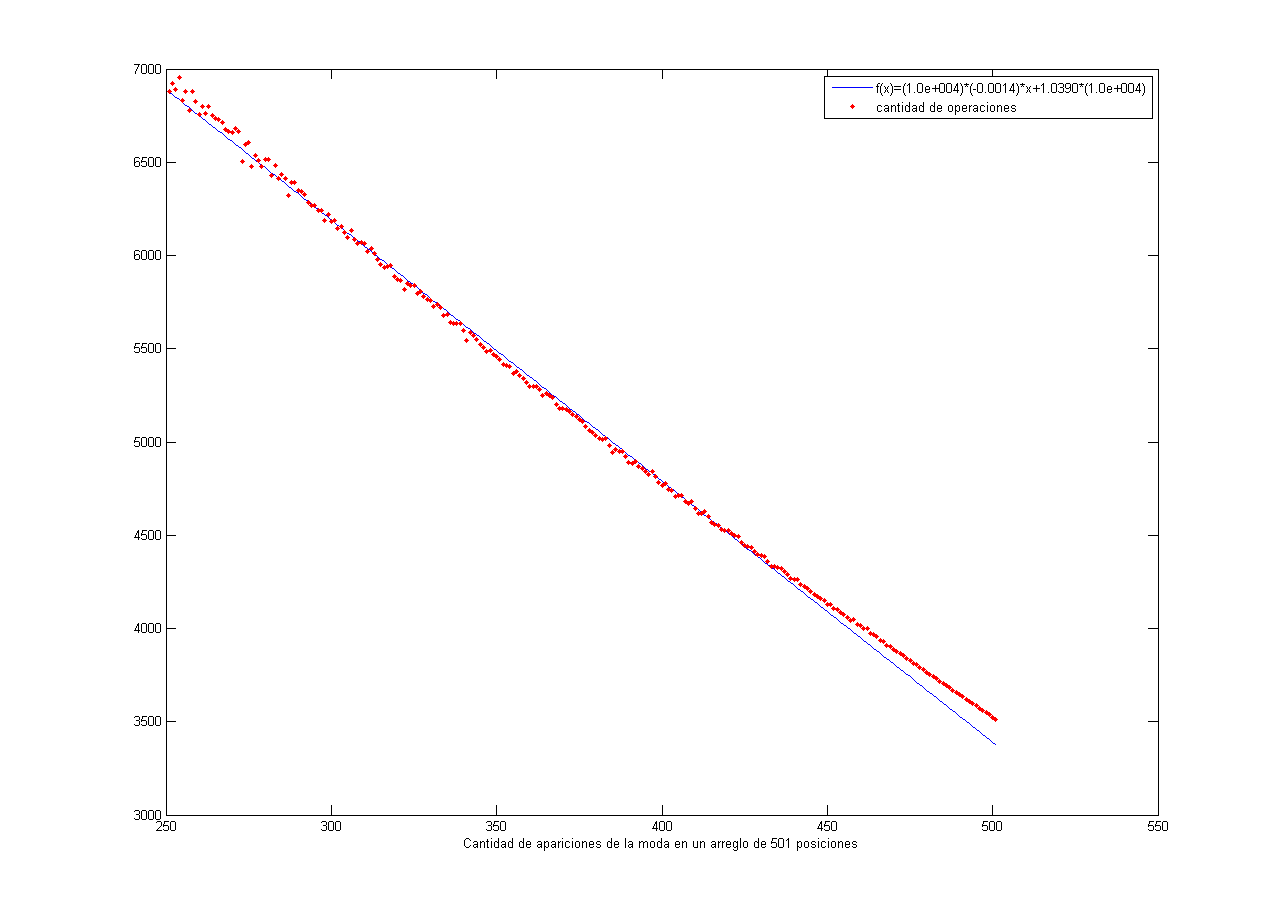
\includegraphics[scale=0.7]{../../codigo/ejercicio3/benchmark/graficos/frecuencia/frecuencia.png}
\caption{Cantidad de operaciones en funci'on de la frecuencia ($n$ = 500)}
\label{Ej3fig2}
\end{figure}

\begin{figure}[H]
\centering
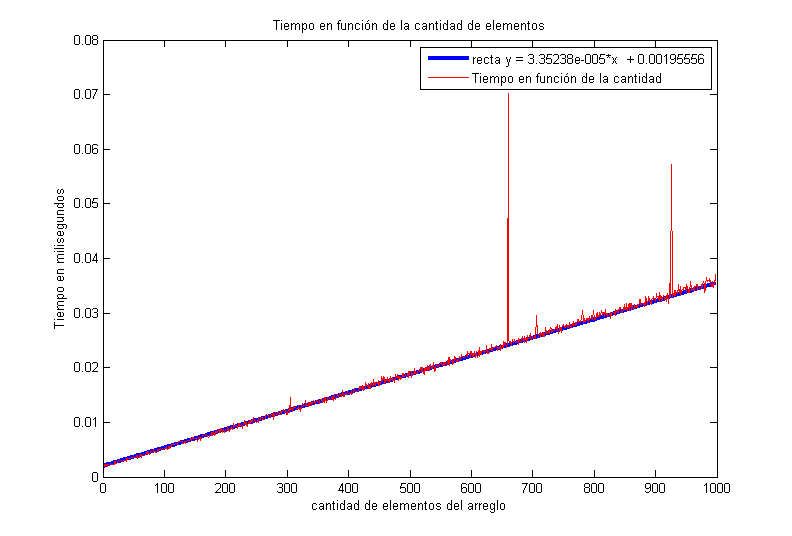
\includegraphics[scale=0.7]{../../codigo/ejercicio3/benchmark_de_tiempo/graficos/moda-1000-casos.png}
\caption{Tiempo (milisegundos) en funci'on del tama\~{n}o del arreglo}
\label{Ej3fig3}
\end{figure}

\begin{figure}[H]
\centering
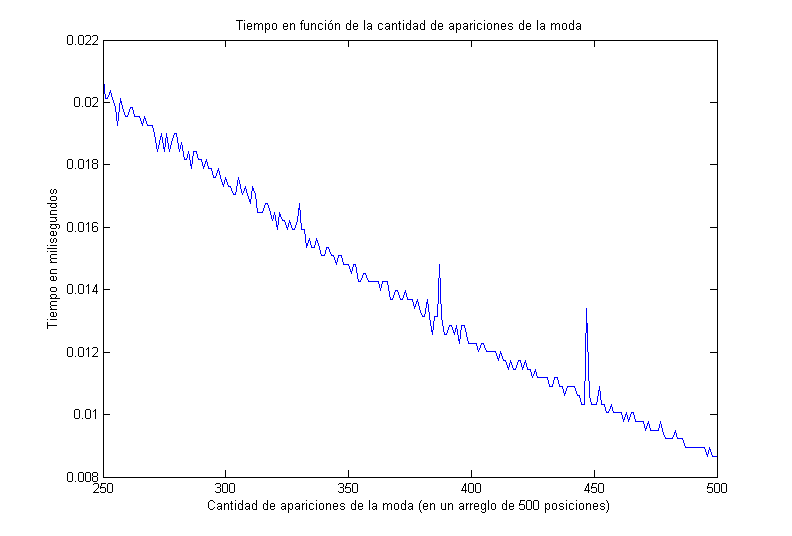
\includegraphics[scale=0.7]{../../codigo/ejercicio3/benchmark_de_tiempo/graficos/aumento-frecuencia.png}
\caption{Tiempo (milisegundos) en funci'on de la frecuencia ($n$ = 500)}
\label{Ej3fig4}
\end{figure}
\newpage
\section{Discusi'on}
\paragraph{}
En el gr'afico de tiempo se observ'o que al aumentar el tama\~{n}o del arreglo, el tiempo 
aumenta de forma lineal. Lo mismo ocurre con la cantidad de operaciones . Esta situaci'on se 
corresponde con el an'alisis te'orico que se realiz'o. 
\paragraph{}
Por otro lado en los gr'aficos en funci'on 
de la frecuencia de la moda, el tiempo y las operaciones parecieran decrecer linealmente. Esto 
evidencia que el mejor caso se produce cuando todos los elementos del arreglo resultan ser la moda. Esto se
explica porque si todos los elementos son iguales a la moda, el $if$ de la l'inea 5 del pseudoc'odigo
siempre tiene una condici'on de entrada falsa, por lo que el ciclo recorre el arreglo sin 
hacer otro tipo de operaci'on. 
\paragraph{}
Para finalizar, podemos decir que el comportamiento que obtuvimos coincidi'o con el esperado.
